\documentclass{article}

\usepackage{graphicx}
\usepackage{tikz}
\usepackage{tikzsymbols}
\usetikzlibrary{calc,patterns,shapes.geometric}
\pagestyle{empty}
\usepackage[margin=0pt]{geometry}
\geometry{papersize={14in,12in}}

\def\centerarc[#1](#2)(#3:#4:#5){\draw[#1] ($(#2)+({#5*cos(#3)},{#5*sin(#3)})$) arc (#3:#4:#5);}

\begin{document}
	\begin{figure}
		\centering
		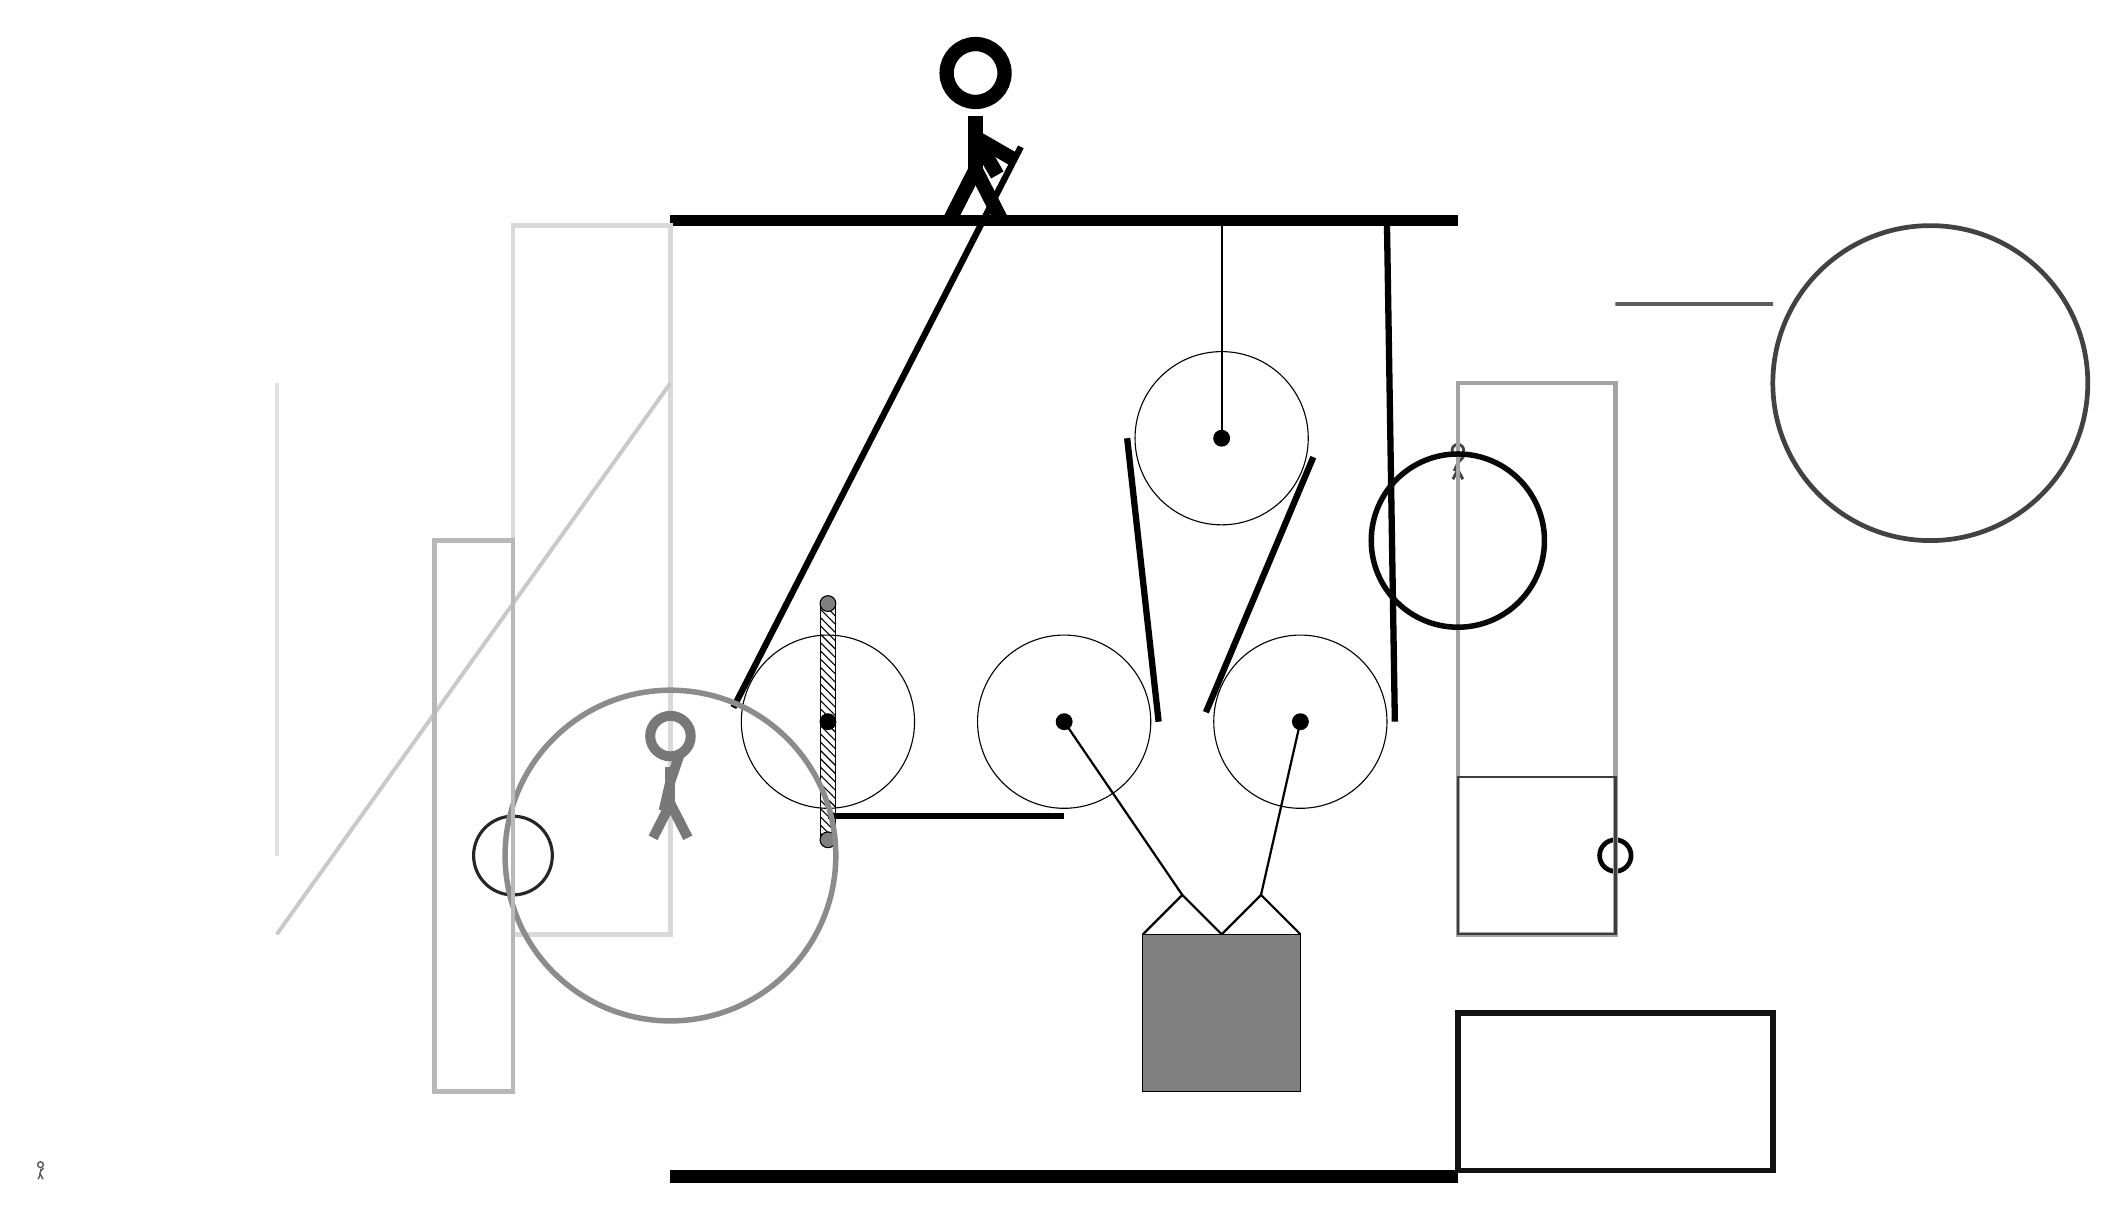
\begin{tikzpicture}
			%%%%% START %%%%%
			
			\draw[fill=black] (-4, 9) rectangle (6, 9.125);
			
			\draw (1, 2.7) circle (1.1);
			\draw[fill=black] (1, 2.7) circle (0.1);
			
			\draw (3, 6.3) circle (1.1);
			\draw[fill=black] (3, 6.3) circle (0.1);
			\draw[thick] (3, 6.3) -- (3, 9);
			
			\draw (4, 2.7) circle (1.1);
			\draw[fill=black] (4, 2.7) circle (0.1);
			
			\draw[thick] (4, 2.7) -- (3.5, 0.5);
			\draw[thick] (1, 2.7) -- (2.5, 0.5);
			\draw[thick]  (2, 0) -- (2.5, 0.5) -- (3, 0);
			\draw[thick]  (3, 0) -- (3.5, 0.5) -- (4, 0);
			\draw[fill=black!50] (2, 0) rectangle (4, -2);
			
			\draw (-2, 2.7) circle (1.1);
			\draw[fill=black] (-2, 2.7) circle (0.1);
			\draw[pattern=north west lines, pattern color=black] (-2.1, 4.2) rectangle (-1.9, 1.2);
			\draw[fill=black!50] (-2, 4.2) circle (0.1);
			\draw[fill=black!50] (-2, 1.2) circle (0.1);
			
			\draw[line width=0.8mm] (0.45, 10) -- (-3.2, 2.88);
			\centerarc[line width=0.8mm](-2, 2.7)(160:270:1.2000000000000002);
			\draw[line width=0.8mm](-2, 1.5) -- (1, 1.5);
			\centerarc[line width=0.8mm](1, 2.7)(270:360:1.2000000000000002);
			\draw[line width=0.8mm] (2.2, 2.7) -- (1.8, 6.3);
			\centerarc[line width=0.8mm](3, 6.3)(-20:180:1.2000000000000002);
			\draw[line width=0.8mm](4.164, 6.06) -- (2.8, 2.82);
			\centerarc[line width=0.8mm](4, 2.7)(160:360:1.2000000000000002);
			\draw[line width=0.8mm](5.2, 2.7) -- (5.1, 9);
			
			\node at (-0.07, 10.2) {\Strichmaxerl[10][120][-30]};
			
			\node[line width=0.2mm, color=black!64] at (-12, -3) {\Strichmaxerl[1][78][47]};
			
			\draw [line width=0.6mm, color=black!98](8, 1) circle (0.2);
			\draw[line width=0.7mm, color=black!93] (6, -1) rectangle (10, -3);
			\draw [line width=0.6mm, color=black!74](12, 7) circle (2.0);
			
			\node[line width=0.7mm, color=black!73] at (6, 6) {\Strichmaxerl[2][65][49]};
			\draw [line width=0.4mm, color=black!85](-6, 1) circle (0.5);
			\draw[line width=0.6mm, color=black!15] (-4, 9) rectangle (-6, 0);
			
			\draw[line width=0.5mm, color=black!12](-9, 1) -- (-9, 7);
			\draw[line width=0.3mm, color=black!11] (7, 3) rectangle (7, 3);
			\node[line width=0.2mm, color=black!53] at (-4, 2) {\Strichmaxerl[7][77][71]};
			\draw[line width=0.5mm, color=black!21](-9, 0) -- (-4, 7);
			\draw [line width=0.7mm, color=black!45](-4, 1) circle (2.1);
			\draw[line width=0.6mm, color=black!36] (6, 7) rectangle (8, 0);
			
			\draw[line width=0.3mm, color=black!76] (8, 0) rectangle (6, 2);
			\draw[line width=0.5mm, color=black!63] (8, 8) rectangle (10, 8);
			\draw[line width=0.6mm, color=black!28] (-6, -2) rectangle (-7, 5);
			\draw [line width=0.7mm, color=black!97](6, 5) circle (1.1);
			
			
			\draw[fill=black] (-4, -3) rectangle (6, -3.15);
			
			%%%%% END %%%%%
		\end{tikzpicture}
	\end{figure}	
\end{document}